\newpage
\thispagestyle{empty}
\mbox{}
\newpage
%------------------/DEBUT DU DOCUMENT/------------------%

\chapter{Transcriptions complètes des 18 langues analysées} \label{chap:ann_trans}

Toutes les transcriptions reproduites ici sont issues des \textit{Illustrations of the IPA} des langues correspondantes.

\begingroup
\sloppy
\section[Afrikaans]{Afrikaans \parencite{wissingAfrikaans2020}\\ \glotto{afri1274}}

{\fontspec{Charis SIL}Ɂɔ pə kiːrət ˈnuərəvənt ən sɔn strəi xəˈkrəi ˈɁuər vi fəˈnələ nəu ˈəintlək di ˈstærkstə vɑs || ˈnɛtu kɔmnaː rə ˈrəisəxər fər ˈbɑi | xəˈɦœl ən əˈlækəˈ vɑrəˈmɑntəl || ˈɦələ bəˈsləitu də di Ɂiən vɑ rət kɑn ˈræxkrəi | Ɂɔ mi ˈrəisəxər tə dʋəŋ Ɂɔms əi ˈmɑntəl Ɂɑf tə ɦaːl | di ˈstærkstə Ɂəs || tu ˈblaːsi vənt ˈɁyːrə lɑŋk fə Ɂɑl vɑ təi vær təs || maːr ɦu ˈɦɑrdər ɦəi blaːs | ɦu ˈdəxtər ɦœl diˈrəisəxər di ˈmɑntəl Ɂɔm ɦɔm || Ɂɛn | tɛn ˈlɑːstə lɑt ˈnuərdəvənt Ɂɑl səi ˈrøːsə ˈpoːxəŋs faːr || tu skəin sɔn ˈlækə ˈvɑrəm || Ɂɛn ˈdaːrlək træ ki ˈrəisəxər sɛː ˈmɑntəl Ɂɑit || Ɂɛn suə mus ˈnuərdəvənt Ɂærˈkɛn | dɑt sɔn di stɛrkstə fɑ ˈnə lə tʋeː vɑs}

%\begin{figure}
%\	\center
%\	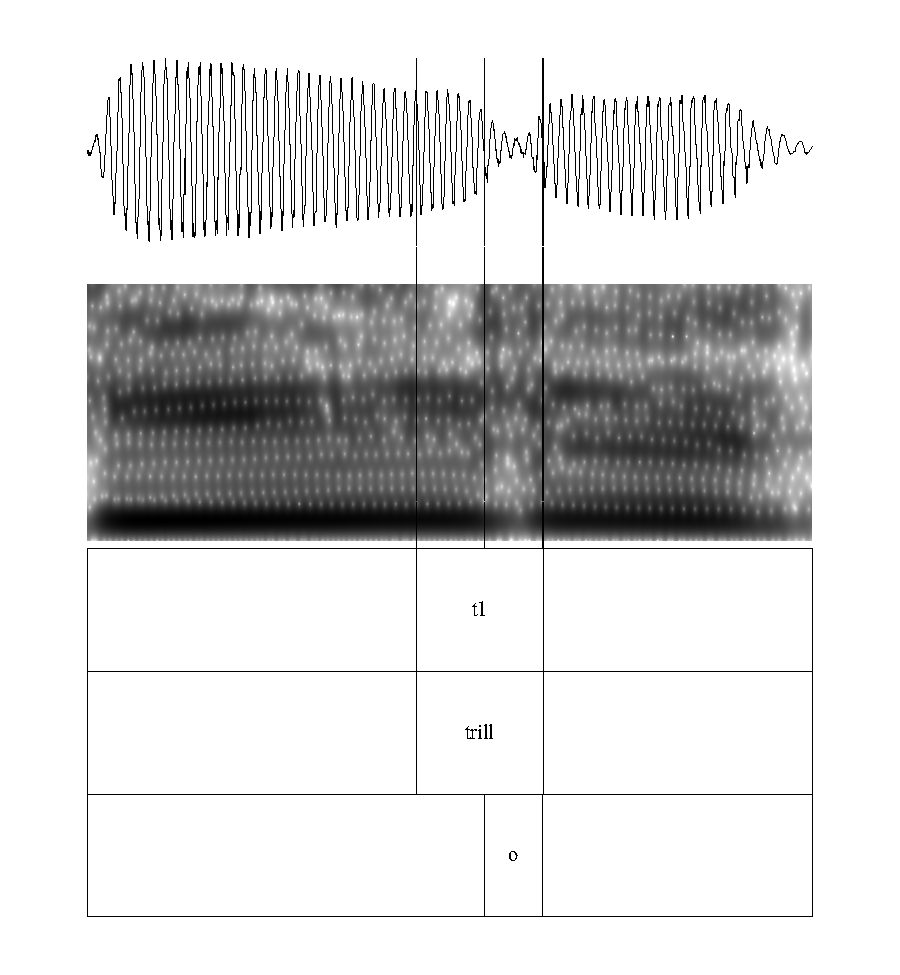
\includegraphics[width=0.45\linewidth]{substance/spectro_images/afri1264_1}
%\	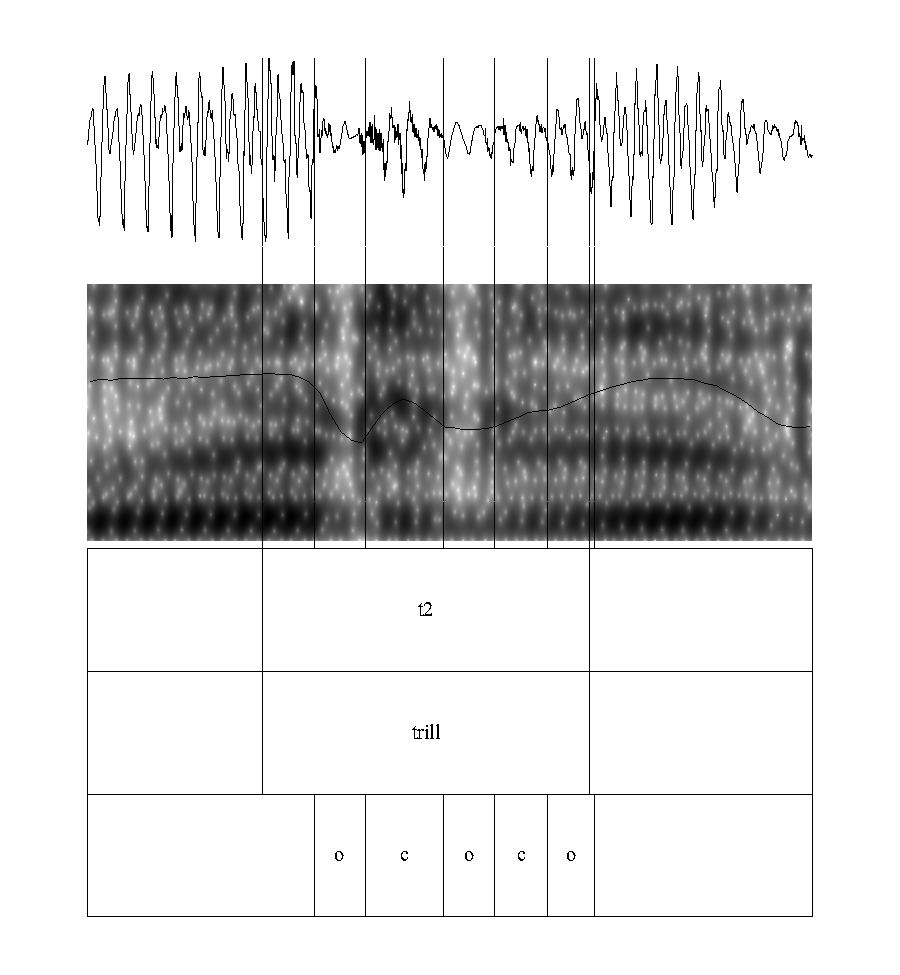
\includegraphics[width=0.45\linewidth]{substance/spectro_images/afri1264_2}
%\	\caption{}
%\	\label{fig:afri12642}
%\\end{figure}

\section[Amarasi]{Amarasi \parencite{edwardsAmarasi2016}\\\glotto{koto1251} }

{\fontspec{Charis SIL}ʔɐw kaːŋkiˑ βi ʔɔmɐ ʔɐw ʔkɔ nɛkmɛsɛʔ ʔɐ̰w̰ ʊ̰ːɐb ʔejk ʔwɐb mɛt̪ɔʔ kɔt̪ɔs ʔɐmɐ ɾasɪ ʔəw h ʊt̪ ɔːn nɔk kʊɐn nɛk mɛsɛʔ nɛkmɛsɛʔ (əw hɔʔ) nəhonɪʔ kɔ nbi nɛkmɛsɛʔ. nɛkmɛsɛ ɾɛʔiɐ ʔʊnʊʔ t̪ɛ nmʊɪʔ kʊˑɐˑn kʊɐn ɐmna̰ːʔ ma na̰ʔ nʊɐ. ʔɛs ɛt̪ ʔa̰t̪ akɐʔ t̪$^\textrm{{\small ʔ}}$akɐʔ ʔɛs ʔɛt̪ kɔt̪ɔs kɔrʔɔt̪ɔ ʔəw mamɐ nɔʔkɐ ʔt̪akɐʔ əw bapɐ nɔʔkɐ kʊɐn ɐmnasɪ̰ʔ rɛʔ abɪt̪ nɛː ʔɔnem ɐ ʔɔɾas iɐ sin nmojn ɛ̰t̪˺ kʊɐn ɛs kan ɛ nɛkmɛsɛʔ}


\section[Espagnol d'Argentine]{Espagnol d'Argentine \parencite{colomaArgentineSpanish2018}\\\glotto{amer1254} }

{\fontspec{Charis SIL}el ˈβjen·to ˈnoɾ·te jel ˈsol dih·ku·ˈti·an so·βɾe ˈkwal ˈde·ʃos ˈe·ɾae̯l ˈmah ˈfweɾ·te | kwan·do pa·ˈsow neks·ˈtɾa·ɲo βja·ˈxe·ɾo̯em ˈbwel·to̯e ˈnu·na ˈaɲ·tʃa ˈka·pa || el ˈβjen·to jel ˈsol kom·bi·ˈnje·ɾon eŋ ke kje ˈnan·teh lo·ˈɣɾa·ɾao̯ βli·ˈɣa·ɾal βja·ˈxe·ɾo̯a ki·ˈtaɾ·se la ˈka·pa se·ˈɾi·a kon·si·ðe·ˈɾa·ðo ˈmah po·ðe·ˈɾo·so || el ˈβjen·to ˈnoɾ·te so·ˈplo koŋ ˈɡram ˈfu·ɾja | pe·ɾo ˈkwan·to ˈma·so ˈpla·βa ˈma·se̯a ɣa·ˈra·βae̯l βja·ˈxe·ɾo ðe suˈka·pa || poɾ ˈfin el ˈβjen·to ˈnoɾ·te̯a βan·do· ˈno lae̯m·ˈpɾe·sa || en·ˈton·seh βɾi·ˈʃo̯el ˈsol ko naɾ·ˈðoɾ | ejn·me·ˈðja·ta·ˈmen·tel βja·ˈxe·ɾo se ðeh·po·ˈxo ðe su ˈka·pa | poɾ lo kel ˈβjen·to ˈnoɾ·te ˈtu·βo ke re·ko·no·ˈseɾ la su·pe·ɾjo·ɾi·ˈða·ðel ˈsol ||}

\section[Biélorusse]{Biélorusse  \parencite{birdBelarusian2020}\\\glotto{cent1954}}


{\fontspec{Charis SIL}pawˈnot͡ʃnɨ ˈvʲet͡sʲer i ˈspraˈt͡ʃalʲisʲæ naˈkont̚ taˈʁo xto z ox bɨw mat͡sˈnʲeiʂ (ɨ̥), kaˈlʲi
jaˈnɨ napatˈkalʲi vanˈdrownʲika zaˈʁornutaʁa uˈt͡sʲɵpɫaʂt͡ʃ. jaˈni paʁa ˈd͡zʲilʲisʲæ ʂto toj z
ix͡ xto ˈpʲerʂɨ prɨˈmusʲi̥t͡sʲ vanˈdrownʲika ˈzʲnʲæt͡sʲ ˈsvoj pɫaʂt͡ʃ i ˈbud͡zʲe lʲiˈt͡ʃɨt͡sːa mat͡sˈnʲeiʂ
(ɨ̥m). taˈdɨ pawˈnoʃnɨ ˈvʲet͡sʲer pad͡zʲˈmuw z̥ usʲæˈje svaˈje ˈmot͡sɨ̥, aˈlʲe ˈt͡ʃɨm ͡mat͡sˈnʲej jɵn
ˈd͡zʲmuw tɨm ˈʂtʃɨlʲnʲej vanˈdrownʲik zaˈxutɨvawsʲæ uˈpɫaʂt͡ʃ. naˈrɛʂt͡sʲe pawˈnot͡ʃnɨ vʲet͡sʲer
paˈk̟ʲinuw svaˈje ˈsprobɨ. taˈdɨ ˈsont͡sa ˈʁorat͡ʃa zaˈzʲːæɫa i vanˈdrownʲik imʁˈnʲenːa znʲæw
pɫaʂt͡ʃ. tak pawˈnot͡ʃnɨ vʲet͡sʲer bɨw ˈvɨmuʂanɨ prɨˈznatsʲ ʂto ˈsont͡sa bɨˈlo mat͡sˈnʲejʂɨm z̥ ʔi̥x
aˈbodvux.}\\


\section[Malais du Brunei]{Malais du Brunei \parencite{deterdingBruneiMalay2017}\\\glotto{brun1243} }

{\fontspec{Charis SIL}masa si a̠ŋɪn utara ↗ | sama si matahaɾi bəta̠ŋkar ↗ | pasal sjapa ja̠ŋ laɡi kuat ↗ || ada tjuɾa̠ŋ pəŋambaɾa data̠ŋ ↘ || djuɹa̠ŋ studʒu sjapa ja̠ŋ dapat˺ məŋɡalkan dʒuba̠h pəŋambaratʊʔ ↗ | jata ja̠ŋ palɪŋ kwat˺ ↘ || sja̠ŋɪn utaɾa pʊn ↗ | mənjʊp skwat˺ kwatɲa ↗ || tapi ma̠kɪn kwat ja məniʊp ↗ | ma̠kɪn ta pula̠ŋ pa̠ŋambaɾatu mamiɡa̠ŋ bana banaɹ dʒuba̠hɲaʔ ↘ || sja̠ŋɪn utaɾa pʊn məŋala̠h ↘ || uda̠h atu si matahaɾi laɡi məmantʃaɹ kwat˺ kwat sampaj pəŋambaɾatu ina tahan ↘ || taɾus ja buka dʒuba̠hɲaʔ ↘ || ʒadi si a̠ŋɪn utaɾa pʊn ↗ | pa̠ksa ŋa̠kʊn si matahaɾi laɡi kwat˺ daɾi kadijaʔ ↘}

\section[Sarde de Cagliari]{Sarde de Cagliari \parencite{mereuCagliariSardinian2019}\\\glotto{meri1242} }

{\fontspec{Charis SIL}su ˈbːentu e ðramunˈtana e su ˈzɔli ˈvianta abːetːiˈendi aˈpːittsuzu e ˈkːini ˈvessi su βruˈfːɔrti | ˈkandu ˈɛst arriˈbːau ˈunu vjadʤaˈɾɔɾi imbusˈsau in ˈdunu manˈteɖɖu || ˈissuzu ˈanti detˈtsiɾju ɣa su ˈβrimu ɣi ˈvessiɾi arrenˈneʃʃu a ˈfːai bːoˈɣai su manˈteɖɖu a su vjadʤaˈɾɔɾi | ˈiaɾˈɛssi ˈstetːju βru ˈfːɔrti de s ˈatru || ˈduŋkaza su ˈbːentu e ðramunˈtana a sulˈlau βru ˈfːɔrti ki βoˈɾiaɾa | ma ˈβruzu ˈissu sulˈlaɾa || pru su vjadʤaˈɾɔɾi si imbusˈsaɾa in su manˈteɖɖu | e a sa ˈvini su ˈbːent e ðramunˈtana ˈaɾi arrinunˈʧau || in ˈtsanduzu su ˈzɔli ɖɖa kːallenˈtau ˈvendi ˈluʒi | e ˈtːotu in ˈduna ˈbːɔrta su vjadʤaˈɾɔɾi si nd ɛbːoˈɣau su manˈteɖɖu || e aˈiʧi su ˈbːent e ðramunˈtana a ˈdːepju aˈmitːi ka de iz ˈduzu su ˈzɔli ˈvia su βru ˈfːɔrti ||}


\section[Espagnol castillan]{Espagnol castillan \parencite{martinez-celdranCastilianSpanish2003}\\\glotto{cast1244} }

{\fontspec{Charis SIL}el ˈβjen̪to ˈnoɾte ʝ elˈsol poɾˈfjaβan soβɾe ˈkwal̪ ˈdeʎoˈs eɾa e̯lˈmasˈfweɾte ǀ kwan̪do̯ aθeɾˈto a̯ paˈsaɾ um bjaˈxeɾo̯ emˈbwel̪to̯ eˈn ãnʲtʃa ˈkapa ǁ kombiˈnjeɾon ẽŋ ke kje  ˈn ãn̪tez loˈɣɾaɾa o̯βliˈɣaɾ al βjaˈxeɾo̯ a kiˈtaɾse la ˈkapa ǀ seˈɾia konsiðeˈɾaðo ˈmas poðeˈroso ǁ el ˈβjen̪to ˈnoɾte soˈplo koŋ gɾaɱ ˈfuɾja ǀ ˈpeɾo kwan̪to ˈma soˈplaβa ǀ ˈma se̯ areβuˈxaβa e̯n su ˈkapa e̯l βjaˈxeɾo ǁ poɾ ˈfin ǀ el ˈβjen̪to ˈnoɾte aβan̪doˈno la e̯mˈpɾesa ǁ ẽn̪ˈton̟θez βɾiˈʎo e̯l ˈsol kon aɾˈðoɾ ǀ e i̯ⁿmeˌðjataˈmẽn̯te se ðespoˈχo ðe  su ˈkapa e̯l βɾaˈxeɾo ǁ poɾ lo ke l ˈβjen̪to ˈnoɾte ˈuβo ðe rekonoˈθeɾ la supeɾjoɾiˈða ðel ˈsol}

\section[Arrernte central]{Arrernte central \parencite{breenCentralArrernte2005}\\\glotto{east2379} }

%\begin{flushleft}

{\fontspec{Charis SIL}ʲlkˈɛiliˌwɨnʲə | ʊˈtəɳʊt̪ənə ɐˈɰəlɐɰəlɐˈkəɾɪdʲˌamɐ | ˈtʲəɾtʲʊˈɭə\textrm{ɻ}ɪnʲɐˈpətʲələŋɐˈɻəməlɐ ||
ɐnʲdʲˈaˑmʊnʲdʲɪdʲəlɛiˈtəl̪əkɐ || ˈɻad̪əɾaˑ ɐŋˈɡəɾəgɐ || ɐˈŋwən̪əlɐˈpəkɐ ˈtʲəɾtʲʊˌɭə\textrm{ɻ}inʲˈan̪ə
ɐnʲdʲˈamʊnʲˈdʲɪdʲɪˌkwʊ\textrm{ɻ}ən̪ə iˑˈlʊl̪ɛlədʲɪgəmbwaˑ\textrm{ɻ}əm$^\textrm{{\tiny ə}}$\textrm{ɻ}ɐ || \textrm{ɻ}a ɪˌkəɭʈɐn̪d̪ˈɔɾɐ
ɐɾˈpən̪ən̪ən̪ɪˈkwʊ\textrm{ɻ}əŋɐ || ʲlkˈɛilɪˌwɪnʲəˈ\textrm{ɻ}əkɐmbaɾɐˈwʊɳɪdʲɪgəˈt̪aˑ ʈɛɾəkɐ ||
iˑnˈdəɾɐn̪d̪ɔˑɾə\textrm{ɻ}əˈwʊɳəkɐ || ˈtʲəɾtʲʊˈɭə\textrm{ɻ}ɪnʲə\textrm{ɻ}ˈakən̪ɐnʲdʲˈamʊnʲdʲɪdʲiˑˈkwʊ\textrm{ɻ}ən̪əlɐ
iˑnˈdəɾɐn̪d̪ˈɔˑrɛiˈtəl̪əŋɐ || ʲlkˈɛiliˌwɪnʲɐ ˈwʊɳəməlɐ ɐɾˈpəɳkəkɐn̪d̪ˈɔˑɾɐ ||
ʊˈtəɳəɭˌanəmɐɾˈtʲə̟ɳəkɐ || ʊˈtəɳə ʊ\textrm{ɻ}ˈɛnpɐn̪d̪ˈɔɾˌɛɾəkə || ʊˈɭə\textrm{ɻ}ənʲə\textrm{ɻ}ˈakən̪ɐ
ɐnʲdʲˈamʊnʲdʲɪdʲɪˈkʊ\textrm{ɻ}ən̪ɐ ɪpˈaɾpɐn̪d̪ˈɔˑɾə iˑˈlʊlˈɛləɭəŋɐ || ʲlkˈɛilɪwɪnʲ ɐŋˈgəkɐ | ʊˈtəɳɐ |
ʊndəɐˈtʲəŋəŋə iˑˈlʲəɳpɪnʲɐn̪d̪ˈɔˑɾɐ}
%\end{flushleft}

\section[Gayo]{Gayo \parencite{eadesGayo2006}\\\glotto{gayo1244}}

{\fontspec{Charis SIL}maˈta ni ˈloː ʊˈɾʊm kuˈju utaˈɾaḁ kuˈjuː utaˈɾaː ʊˈɾʊm ˈmaːta nˈloː pəˈloloː saˈɾaː ˈloː || saˈhan si
paˈlɪŋ ˈbəp̚ | kətiˈkɤ saˈɾaː dʒəˈmaː muɾanˈtoː | ˈgɛh ˈʊɾʊm baˈdʒuː pəˈsam || ˈpakea səˈpakat̚
| bahˈwaː sahan si ˈŋok̚ muluˈahni baˈdʒuː pəsamˑˈeaː | ijaŋap̚ paˈlɪŋ ˈbəp̚ aˈɾiː si rɔ̯ˈawaː ||
rəˈɲəl̪ kuˈjuː utaˈɾaː bəɾəˈmʊs sək$^\textrm{ə}$ɾaskrasˑˈe̝ː || ˈtapɪ maˈkɪn ˈkras ˈwɛː bərˈmʊs maˈkɪn
ˈkras dʒəˈma muˈɾanto mulɪˈlɪtniː badʒujˈejaː || ˈdən ahɛˈɾɛː | kuˈjuː utaˈɾaː kaˈlah || ˈmata
nˈloː muˈlɔi pɔˈɾak | rəˈɲəː dʒəˈma muɾanˈtoa muluˈahniː baˈdʒuː pəsamˑˈe || rəˈɲəl̪ kuˈjuː
utaˈɾaː muŋaˈkui | bahˈwaː maˈtaː n$^i$ˈloː ləˈbɪh ˈbəp̚ aˈdɪh kuˈjuː utaɾaˈwaː}

\section[Basque Goizueta]{Basque Goizueta \parencite{hualdeGoizuetaBasque2010}\\\glotto{basq1248} }

{\fontspec{Charis SIL}ipàr ai̯s̻éaǀ ta ḛ̀u̯s̻kiaǁ\\
ipàr ai̯s̻éaǀ ta ḛ̀u̯s̻kiaːǀ indàrts̺una s̻èi̯n ts̻en ʔés̺pan ài̯ s̻iála ǀ iβ́ltaɾi βa pas̺átu s̻en ǁ
kàpa loði βátem bilʲdúa ǁ ʔeɾ̞áβakʲ(i) s̻utén ǀindàrts̺una is̻ái̯n ts̻ela ǀ
iβílʲtaɾiɾi ǀ kàpa ʔau̯réna ken(d)ùs̻its̻en ts̻ína ǁ 
ʔórdun ǀ ipar ais̻ék ǀ b̥eɾ̞̀ íɲal ɣus̻ìkin ɟó s̻un ǁ biɲo s̻émbat eta fu̯érteo ʝó ǀ ibílʲtaɾik ǀ
órðun eta es̺túo ʔèus̺ten ts̻in beɾé kàpaɾi̻ ǁ
ʔḁs̻kénen ipàr ais̻ék ǀ e̥ts̺ì̥ta ǀ uts̻ì ín ts̻un beɾ̞aléi̯ ɲa ǁ
géɾ̞o ǀ èu̯s̻ki̯a fu̯èrte βeɾòts̻en as̺í s̻en ǁ
ta̰ ḭβílʲtaɾik ǀ béleʃe ken(d)ú s̻um beɾé kḁ̀pḁ ǁ
ta̰ óla ǀ ipàr ai̯s̻ék a̰i̯còrtu βar is̻an ts̻ún èu̯s̻kḭa̰ s̻éla bìetan indà̰r̥s̺u̥n̥ḁ ǁ}

\section[Indonésien Bajau]{Indonésien Bajau (Lombok de l'est) \parencite{archangeliIndonesianBajauEast2019}\\\glotto{indo1317}}

{\fontspec{Charis SIL}mataɦari bɯkɯ saŋai utɯɾɯ || tɕɯɾitɯ itu dimulai ma sə̥bua̤ kampa̤
dikːɪʔ || nia ʔaɦa lɯlːɯ makai dʑakɛt təbːal || ma atas laŋiʔ | nia
mataɦaɾi bɯkɯ saŋai utɯɾɯ || mataɦaɾi bɯkɯ saŋai utɯɾɯ itu muɣai
lɔmbɯ | lɔmbɯ sai saʔ paliŋ bagam kəkuataŋ nɯ ||
lɔmbɯ nɯ  iɾu təntaŋ sai sai saʔ kole mugai ʔaɦa lɯlːɯ
iɾu ləbanaŋ nɯ dʑakɛt̚ nɯ || saŋai utɯɾɯ ɲɔbanaŋ pɯɾtamɯ
ʔai a̰i saʔ kole mugai a̤ɦa lɯlːɯ iɾu ləbanaŋ nɯ dʑakɛt̚
nɯ || ɲɔbanaŋ jɯ pəlua nɯ kəkuataŋ nɯ || saŋai saʔ
agaʔ bagal plua nɯ || pɯɾɯ pɔɦɔŋ pɔɦɔŋ iɾu bəɾgɔjaŋ kɯ̰
utɯɾɯ || bauŋla̤ɦ jɯ | kole ku muɣai a̰ɦa lɯlːɯ iɾu
ləbanaŋ nɯ dʑakɛt̚ nɯ || tapi a̰ɦa lɯlːɯ iɾu numalaŋ
bɯkɯ masi jɯ makai dʑakɛt̚ nɯ || məɾɯsɯ jɯ dʑəɾənːi
badaŋ nɯ le saŋai iɾu || jɯmɯnɯ tətːaʔa̰ jɯ makai
dʑakɛt̚ nɯ ɲɔbanaŋ pɔɦɔŋ bɯkɯ ʃal a̰ha lɯlːɯ iɾu bəɾgɔjaŋ ||
tapi tətːa a̰ha lɯlːɯ iɾu makai dʑakɛt̚ nɯ || aɦɪɾnɯ
məɲəɾa̤ɦla̤ si saŋai utɯɾɯɯ̰ iɾu || təɾus mataɦaɾi ɲɔbanaŋ
kəkuataŋ nɯ || pr̥tɯmɯ | pəlua nɯ panas saʔ gai
təɾlalu panas || aɦa lɯlːɯ iɾu mulai ŋəɾɯsɯ panas || tapi masi
jɯ makai dʑakɛt̚ nɯ || ɲɔbanaŋ jɯ lagi untuk kədua kali
nɯ || mataɦari iɾu pəlua nɯ panas saʔ ləbi̤ bagal daɾi saʔ
pəɾtəmə nə iɾu || aɦa lɯlːɯ iɾu kəpanasaŋ jɯmɯnɯ
ləbanaŋ nɯ dʑakɛt̚ nɯ || dadi mataɦari saa̰ dadi
pɯmɯnaŋ nɯ}

\section[Itunyoso Trique]{Itunyoso Trique \parencite{dicanioItunyosoTrique2010}\\\glotto{sanm1298}}

{\fontspec{Charis SIL}na3ne1 kːiɦ3 n̤ĩ2 kʷi3 ũ3nũʔ3 nu2kʷe3 nĩʔ4 s̬i3s̬i2 ũ3 ŋõʔ2ŋõʔ2 nũʔkʷ e2 nu1kʷ aɦ3
t̬o3 βa32 ja3 ka4ʃĩ43 ŋõ2 jũ4$^\textrm{\small ʔ}$ũh3 ne2ke2 ŋo2 ɽe̞3to32. nĩ2 ka3βi3 ka3ʔmĩ32 nũ2kʷe3 
ŋga13-nĩ2 a4taɦ3 nũ2k̬ʷe3 si3s̬i2 ta1 βa32 ũ3 ŋõʔ2-ŋõ2 nũ2k̬ʷeʔ2 ki3ʔjaɦ4 as2-nĩ3j̃ə̃3
ka̰3ne3 jũ4ũɦ3 tʃa1na1 ta3 ɾe3to32 ne2$^\textrm{\small h}$ke2ũɦ3 nĩ2 βeʔ4 k̬a3̃βĩ si3-nu1kʷaɦ3 to̤3
βa32. nĩ2 ka3tʃi1 na3ne1 ka3$^\textrm{\small ʔ}$jə̃3 $^\textrm{\small n}$da2-te̞3$^\textrm{\small ʔ}$e3. ta2si3 ta2-te3e3 a4$^\textrm{\small ʔ}$jə̃ɦ4 na3ne1 t̬a3 
sa3ni2 ta1-te3e3 nã3nə̃2ə̃2 jũ4$^\textrm{\small h}$ũh3 tʃa1na1 t̬a3 mə̃̆3ʔə̃3-ũ3 ŋga1 re3to32 ne2$^\textrm{\small h}$k e2-
ũ3. sa3ni2 t̬a3r̥ku2 nĩ2 ka3$^\textrm{\small ʔ}$nĩʔ3 ɾa43 na3ne1 ta3 s̬i3 ka2$^\textrm{\small h}$j̃ə̃3. ŋa13-nĩŋ2 kʷi3 kḭ3jaɦ3
ta2rə̃ŋ32 ka3naʔ3 nə̃4. ŋga13-nĩ2 ta2-kʷɔ3kʷə̃ʔ3 ka̰4ʔne ɦ4-ṳ̃3 re3to32 tʃi3ɾaɦ5-ṳ̃3
ki3$^\textrm{\small ʔ}$a3. ta13 ka3mĩ3 t̪a3 ka3ɾa3 tʃi3na32 na3 ne1 kːiɦ2 t̪a3 si3s̬i2 nũ1kʷ aɦ3 to3 kʷi3
ɾjə̃ɦ3.}\\

\textit{Note : Dans la transcription de DiCanio, les tons sont représentés en indice.}

\section[Kazakh]{Kazakh \parencite{mccollumKazakh2020}\\\glotto{kaza1248}}

{\fontspec{Charis SIL}bɪr̪ kʰʏ̆n̪ɪː s̪oˑɫt̪st̪ɪk ʒi̯͡el̪ mi̯͡en̪ kʰʏn̪ i̯͡ekʰjʏ͡w ɑr̪ɑɫaɾn̪̩d̪æˑ kʰɘm͡ məχt̪ɪ̆ i̯͡ekʰi̯͡e n̪n̪̩ ʃi̯͡eʃi̯͡e ɑɫmaj ǀ bæs̪ekʰi̯͡el̪es̪i̯̰͡ḛd̪ɪ̆ ǁ d̪æl̪ ɔ̟s̪ɪ̆ mi̯͡ez̪i̯͡et̪t̪i̯͡e ʒoɫ bojin̪d̪æː ʃɑpɑɴɢ ɑ͡oˑɾan̪ɪ̆p kʰi̯͡el̪i̯͡e ʒɑt̪̚qɑn̪ ʒoɫɑwʃə̆n̪ɘ̆ kʰi̯͡ez̪ɪk̚t̪ɪɾi̯͡ed̪ɪ ‖ i̯͡ekʰj͡ʉwɪn̪j͡e ŭ͡oj kʰi̯͡el̪i̯͡et̪̚ ǀ kʰɘm d̪i̯͡e kʰɘm ʒoɫowʃə̆ʀɑː s̪t̪n̪̩d̪i̯͡eɣɪ ʃapɑn̪n̪̩ ʃi̯͡eʃkɪz̪i̯͡e ɑˑɫsɑ̰ː ǀ s̪oˑɫ məχt̪ə d̪i̯͡eɣi̯͡en̪ ʃi̯͡eʃɪ̆mɡḛ ki̯͡el̪i̯͡ed̪ə̆ ǀ s̪oɫt̪s̪t̪ɪk ʒi̯͡el̪ ǀ bɑːr̪ kʏ̆ʃʏmi̯͡e̪n ʒi̯͡el̪ ʏɾl̪i͡j βɜˑst̪ajd̪ɪ ǁ oɫ qɑːt̪̚t̪ə͡ ʏ̆r̪li̯͡eɣi̯͡en̪ s̪ɑjə̃n̪ ʒoɫɒwʃə̆ ʃɐ̆pɑn̪n̪ɑ oɾɑn̪ɑ t̪s̪i̯͡ḛ̹d̪ɪ̰ ǁ ɑmɑˑɫə t̪ɑwsɫ̩ʁɑn̪ s̪oɫst̪ʰʏk ʒi̯͡el̪ ǀ kʰi̯͡ez̪i̯͡ekt̪ə kʉn̪͡ŋɡi̯͡e bi̯͡eɾd̪ɪˑ ǁ kʏn̪ ʒɑːr̪qə̆r̪ɑːp̚ ʃəʁəp ʃoɫowʃn̪əŋ s̪t̪n̪i̯͡e n̪əɾn̪̩ ʃɐ̥ʃɑˑ βɐs̪t̪aʀan̪d̪æː ǀ kʏ̆n̪͡ n̪ʊɾən̪ɑˑ ʒəɫɴ̩ɢɑːn̪ ʤoɫɑwʃə ǀ ʏ̆s̪t̪n̪̩d̪i̯͡eɡɪ ʃɑ̆pʰɑn̪n̪̩ ʃɪʃi̯͡ḛd̪ɪ̰ˑ ǁ oˑs̩ʊ͡ oˑq͡χɨʁɑd̪ɑˑn̪ kʰi͡jn̪̩ ǀ s̪oɫt̪s̪t̪ʰʏ̆k ʒi̯͡el̪ɪ kʰʏ̆n̪n̪ɘŋ u̯͡ɵzn̪i̯͡en̪ məχt̪ɛ̆͜ ͡i̯ekʰi̯͡en̪ɘn mojn̪̩d̪ɑwʁɑˑ t̪ʰṵɾɑ̰ kʰi̯͡ḛl̪d̪ɪ̰ˑ}

\section[Mavea]{Mavea \parencite{guerinMavea2009}\\\glotto{mafe1237}}

{\fontspec{Charis SIL}ˈnao̯ | ˈnao̯ taˈm̼aːku || ma moˈlulvoː || ˈamːa moˈlulvo roː moˈto moˈv̼a 
sur poŋ aˈite ro$^\textrm{\tiny ʔ}$ ˌmov̼anˈv̼aːno moˈsi ˌmom̼aˈsuːr || aˈlao na ˌtas
ˌmo-m̼aˈsuːr m̼aˈtan tiˈnaːra || məs ˌmom̼aˈsuːr m̼aˈtan tiˈnaːra ro || ˌmolp̼arˈp̼aːra 
ro ˈmoːnːeː || ə k̚ || ˈmon kaˈkato ˈɸoːko aˈite m̼aˈtan ˈamːa ro kaˈkato ˈβoːko 
moˈdeːre | ˈmeːre || kaˈkato ˈvoːko moˌsopoˈtea kaˈkato βiˈriːe na || ə ˈtaːro ro 
ˈmaːma ˌmom̼aˈsuːr moˈsi | ˌmolop̼arˈp̼aːra v̼a m̼aˈtan tiˈnaːra ro ˈmoːn kaˈkato 
ˈɸoːko aˈite ro ˌmoːn kaˈkato ˈβoːko ro | ˈmeːv ro$^\textrm{\tiny ʔ}$ || kaˈkato ˈβoko moˈtapair 
ˈmaːma ro moˈteːte || ˈteːte nə ˈmaːma moˈsaːima | m moˈsaː || rm̩p̩m̩ ˈmaːma moˈm̼elˌtapul
moˈsaːima || moˈsa moˈpoŋ moˈsuruvu ro ˈmon ma || ˈ tamleˌseː aˈite ˈmom̼a ro moˈvaraɪ̯a 
nːa ˈmovə || ˈnːo nel naˈpar koˈm̼a ˌkolp̼arˈp̼aːra ||}

\section[Sasak]{Sasak, dialecte du Meno-Mené \parencite{archangeliSasakMenoMeneDialect2020}\\\glotto{nort2820}}

{\fontspec{Charis SIL}ʥəlo kaɲʨə ʔaŋin dajɨ bəsiaʔ kiɾɨ kiɾɨ sai kuata ||
muʔ təɾus liwa dəŋan kadu ʥakɛ || ʥəlo kaɲʨɨ ʔaŋin b̥səpakat
saisai tao piəʔ dəŋan nu bukaʔ ʥakɛt | iɨ wah
məna || muʔ təɾus ʔaŋin mulai niup ʥaŋkə ləlah | laɡuʔ dəŋan
nu seɾen ãtuʔ ʥakɛtən siʔ təlihən || kɔntɛʔ ʨəɾitɨ | ʔaŋin
ɲəɾah || muʔ təɾus ʥəlo pəŋɡitaan kaɲʨə sinan saʔ panas
| muʔ laŋsuŋən bukaʔ ʥakɛtən || muʔ təɾus ʔaŋin
ŋakun ntan ʥəlo iə kuata ||}

\section[Seenku]{Seenku \parencite{mcphersonSeenku2019}\\\glotto{nort2820}}

{\fontspec{Charis SIL}mô̯aː d͡ʒî̯o fóː lɛ̂ː ʃú wɛ̀ mɔ̃̀mɛ̃̀ːn tè t͡sɘ̋-kɛ́ ꜜsɔ̋n-ta̋ te̋.
fóː lɛ̂ː ʃú wɛ̀ mɔ̃̀mɛ̃̀ːn tè tsɘ̋-kɛ́ ꜜsɔ̋n-ta̋ ꜜ ʃĩ̋ː ʃí kũ̯̋ĩ̋ː nɛ̋ ʔȉ fə̏ŋã̂lɛ́ ʃĩ̀ nɛ̋ főn tə́rɛ̃́ nɛ̏.
ɡȕ̯ɔ-nɛ̃́ -kâ lɛ̏ ʃúű jí-ꜜnáː íː mã̀ːntɔ̃̀m blè dzḭ̋ mi̋́ꜜwɛ̋ í tȁ fĩ̀ɛ̃ ꜜwɛ̋.
ȉ lȅí̯ bïː tə́ɾɛ́ nɛ̃̋ ʃí̯ɔ nɛ̃̋ mȁ màːntɔ̋m bɛ́ bȕ̯ɔ ɡȕ̯ɔ-nɛ̃́ -kà́ wɛ̀.
fóː lɛ̂ː ʃú wɛ̀ mɔ̃̀mɛ̃̀ːn tè lɛ̏ b͡βú̯ɔ fə̏ŋã́ã̀ wɛ̀.
ȁá sĩ̀ nɛ̋ bû̯ɔ nɛ̏ fə̏ŋã́wɛ́ ɡȕ̯ɔ-nɛ̃́ -kâ léi̯ mã̀ːntɔ̃̀wɛ̀-kɔ̃̀ ʔí wɛ̋.
fóː lɛ̂ː ʃú wɛ̀ mɔ̃̀mɛ̃̀ːn tè lȅ́ dȁn-kȕ nɛ̃̏ -ɟə̏ɾȁn-ɟə̏ɾȁ.
sɔ̋n-ta̋ lɛ̏ b͡βú̯ɔ ɡú̯ɾû mà bɛ̀ ɡȕ̯ɔ-nɛ̃́-kâ lȅ́ mã̀ːntɔ̃̀m bɔ̀ í wɛ̋.
fóː lɛ̂ː ʃú wɛ̀ mɔ̃̀mɛ̃̀ːn tè ꜜlè bȉːʔḭ̏ ꜜsɔ̋n-ta̋ nɔ̃̋ŋ kɛ́ ʃȉ̯ɛ-bɛ̏ íwi̋ fĩ̋n dɡǔaː.}

\section[Tamambo]{Tamambo \parencite{riehlTamambo2005}\\\glotto{malo1243}}

{\fontspec{Charis SIL}ˈlaŋĩ ˌmanã ˈalo nãˈloli mãtʰan hiˈseɪ mõˈswiɣa, tʰamãˈlohi haˈtʰea ˈmõm le ˈtʰusi
mõˈruru nã ˈruru ˌvonõˈɣaɣa. nãˈsorˌasoˈrahi hiˈseɪ mõˈlol nã ˌtʰamãˈlohi mõl tʰaˈkai
nõnã ˈruru ˈro ˈnĩa ˌmãra ˈswiɣa. mõˈiso ˈlaŋĩ mõˈsere mõˈswiɣa mõtʰa ˈsere
mõˈswiɣa ˈtʰinã ˌtʰamãˈlohi  mõˈtʰaʊri laˈlat nõnã ˈruru mõˈiso mõˈswiɣa. mõˈiso
ˈalo mõˈalo mõˈswiɣa, ˌmõtʰe ˈtʰwaɪ ˌtʰamãˈlohi mõl tʰaˈkʰaɪ nõnã ˈruru. mõˈiso ˈlaŋĩ
mõviˈtʰia tʰeˈleɪ ˈalo ˈmõre ˈnĩho ˌmãra ˈswiɣa.}

\section[Ukrainien]{Ukrainien \parencite{pompino-marschallUkrainian2017}\\\glotto{sout2604}}
{\fontspec{Charis SIL}
ɔdˈnɔɦɔ ˈrazu | pɔspɛrɛˈt͡ʃaɫɪsʲa ˈsɔnt͡sɛ ipʲiu̯ˈnʲit͡ʃnɪi̯ ˈʋʲitɛr ˈs‿prɪwɔdu ˈtɔɦɔ |
ˈxtɔ znɪɣˈdwɔxsɪlʲˈnʲiʃɪi̯ || aʒˈraptɔmwɔˈnɪ | pɔˈmʲitɪɫɪ mandrʲivnɪˈka | jɜ ˈkɪi̯
ˈsamɞ prɔˈxɔdɪu̯ pɔu̯znɪx | ˈkutajuʃɪsʲ upalʲˈtɔ || ɔˈbɪdʋadʲii̯ˈʃɫɪ ˈsʲpʲilʲnɔji
ˈdumkɪ | t͡ʃə ˈtɔi̯ ˈbudɞˈʋɪznanɪi̯ sɪlʲˈnʲiʃɪm | ˈxtɔˈʋɪmusɪtʲ mandrʲivnɪˈka
ˈzʲnʲatɪ swɔˈjɛ palʲˈtɔ || pʲivˈnʲit͡ʃnɪi̯ ˈʋʲitɛrduu̯ zusʲiˈjɛji ˈsɪɫɪ | aˈɫɛ t͡ʃɪm
ˈduʒt͡ʃɛ vʲin duu̯ | tɪm ʃɪlʲˈnʲiʃɛ ˈkutau̯sʲa mandrʲivˈnɪkuswɔˈjɛ palʲˈtɔ ||
u̯ˈrɛʃtʲi ˈrɛʃtpʲivˈnʲit͡ʃnɪi̯ ˈʋʲitɛrpɛrɛˈstau̯ bɔˈrɔtɪsʲa || i ˈtut ˈsɔ̃nt͡sɛ zʲiɣˈrʲiɫɔ
pɔˈʋʲitrʲaswɔˈjimɪ prɪvʲitnɪmɪ ˈprɔmɛnʲamɪ | i‿u̯ˈʒɛ ˈt͡ʃɛrɛz ˈdɛkʲilʲka xʋɪɫɪn |
mandrʲivˈnɪɡ zʲnʲau̯ swɔˈjɛ palʲˈtɔ || ɔˈtɔʒ | pʲiu̯ˈnʲit͡ʃnɪi̯ ˈʋʲitɛr ˈʋɪmuʃɛnɪi̯ ˈbuu̯
ˈʋɪznatɪ | ʃə ˈsɔnt͡sɛˈs‿pɔmʲiʒ nɪɣ ˈdvɔx | buˈɫɔ sɪlʲˈnʲiʃɪm}


\chapter[QR codes redirigeant vers les chansons des chapitres]{QR codes redirigeant vers les\\chansons des chapitres}\label{chap:ann_qrcode}
\endgroup

Les QR codes présents dans cette annexe sont présents dans la version numérique sous forme d'hyperliens au niveau des épigraphes de chaque chapitre.

\section{Chapitre 1 - {\cjkfont 歯茎ふるえ音}}

\begin{figure}[H]
	\centering
	
\includegraphics[width=0.3\linewidth]{qr_codes/japanese_song}
	\caption{\href{https://www.youtube.com/watch?v=aLVMmgviTGU}{\textg{Bremen}} est une chanson en japonais de Guernica sortie en 1982 dans l'album \textit{Kaizo Heno Yakudo}.}
	\label{fig:japanesesong}
\end{figure}

\section{Chapitre 2 - {\cjkfont 치경 전동음}}

\begin{figure}[H]
	\centering
	
\includegraphics[width=0.3\linewidth]{qr_codes/korean_song}
	\caption{\href{https://www.youtube.com/watch?v=m-SvT47Vfbc}{\textg{On The Street}} est une chanson en coréen de 
			Kim Kwang Seok avec Sang Ji Koh sortie en 2016 dans l'album commémoratif \textit{Kim KwangSeok, Again ({\cjkfont 김광석, 다시}\textit)}.}%
	\label{fig:koreansong}
\end{figure}

\section{Chapitre 3 - {\cjkfont 齿龈颤音}}

\begin{figure}[H]
	\centering
	
\includegraphics[width=0.3\linewidth]{qr_codes/chinese_song}
	\caption{\href{https://www.bilibili.com/video/BV19f4y1W7Qu/}{Ce morceau} est chanté dans le dialecte de Danyang, parlé au centre de la Chine.}
	\label{fig:chinesesong}
\end{figure}


\section{Chapitre 4 - {\telugufont అల్వియోలార్ ట్రిల్}}

\begin{figure}[H]
	\centering
	
\includegraphics[width=0.3\linewidth]{qr_codes/telugu_song}
	\caption{\href{https://www.youtube.com/watch?v=Aa0mWwl1Tp4}{\textg{Rangamma Mangamma}} est une chanson en télougou de MM Manasi, présente dans le film \textit{Rangasthalam} sorti en 2018.}
	\label{fig:telugusong}
\end{figure}

\section{Chapitre 5 - альвеолярный дрожащий}

\begin{figure}[H]
	\centering
	
\includegraphics[width=0.3\linewidth]{qr_codes/russian_song}
	\caption{\href{https://www.youtube.com/watch?v=Iary3X3Vyp0}{\textg{ЦОЙ УМEP!}} est une chanson en russe de МодеМ sortie en 2020 dans l'album \textit{Цой умер - Single}.}
	\label{fig:russiansong}
\end{figure}

\section{Chapitre 6 - {\thaifont เสียงรัว ปุ่มเหงือก}}

\begin{figure}[H]
	\centering
	
\includegraphics[width=0.3\linewidth]{qr_codes/thai_song}
	\caption{\href{https://www.youtube.com/watch?v=uOHguUMnQkQ}{{\thaifont หนุ่มน้อย}} est une chanson en thaï de Pongsit Kampee, compilée dans l'album \textit{Kampee Pleng Rak, Vol. 1} sorti en 2014.}
	\label{fig:thaisong}
\end{figure}


%------------------/FIN DU DOCUMENT/------------------%